\section{Introduction}
\label{sec:intro}

A graph index and its search budget jointly determine the quality and cost of approximate nearest-neighbor search (ANNS). Hierarchical Navigable Small World (HNSW) graphs and Vamana make this tradeoff central to efficient vector retrieval~\cite{malkov2020hnsw,subramanya2019diskann}. Index maintenance changes one side of this contract. Even with the same vectors and query, construction order and randomization can change the traversed graph; after data refresh, both the graph and nearest-neighbor ground truth can change. A budget retained from an old index therefore needs its own portability assessment.

The operational question is not simply whether rebuilding changes average recall. A service may require a high fraction of queries to reach a specified recall, while an efficient policy fails that requirement on a subset of requests. We measure the probability of $\rec@10<0.95$: because recall is discrete, one missing neighbor is a failure. A 5\% query-risk limit asks that at least 95\% of queries recover all ten neighbors. It differs from mean recall of 0.95 and from expected missed-neighbor fraction.

Our study separates two forms of evidence. First, on unchanged collections, we transfer a query's retrospective first-passing action from one graph build to another. This measures how the search response changes, without involving TCP or a learned budget predictor. Across four hnswlib/Faiss--dataset combinations, target failure exceeds the target-specific reference by 17.17--23.60 percentage points. Second, we study an executable history-pool policy after 5\% data refresh and rebuilding. Holding that policy fixed, old-to-new risk rises from 3.77\% to 6.69\% on SIFT-100K and from 3.19\% to 7.24\% on Arxiv-Nomic-100K. Figure~\ref{fig:overview} places these different comparisons side by side.

\begin{figure*}[t]
\centering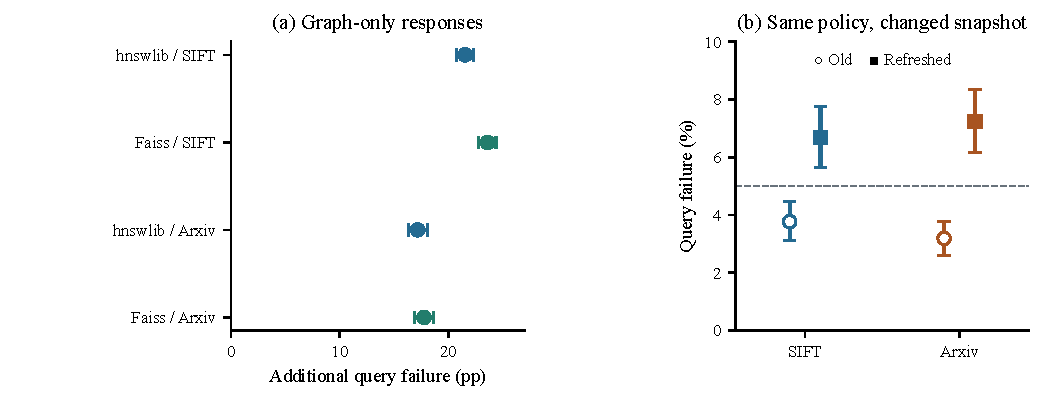
\includegraphics[width=\textwidth]{figures/overview.pdf}
\caption{Two distinct portability tests. Left: graph-only transfer of retrospective first-passing actions; additional failure above each target's own first-passing reference, with 95\% query-cluster intervals conditional on 24 builds. Right: the same executable history-pool policy on matched old and 5\%-refreshed builds; average query risk over ten builds, with crossed target-build/query 95\% intervals. The old/new difference changes both graph and data. Neither comparison treats directed build pairs as independent trials.}
\label{fig:overview}
\Description{Four graph-only incremental-risk estimates are positive. In the separate refresh test, old-policy risk increases on both datasets, crossing the 5 percent line.}
\end{figure*}

\emph{Index-Conditioned Budget Audit} (ICBA) connects these measurements to a serving decision. It identifies the permitted observations, fixes the failure event, isolates policy selection from certification, includes fallback in completed outcomes, and prices information acquisition. Its role is to prevent three distinct quantities from being interchanged: an observed recall improvement, a statistically qualified action, and a net economic benefit.

\emph{Target-calibrated pooling} (TCP) is the recovery case within this audit. It takes historical budgets for the same query, pools them conservatively, and chooses a global grid shift using target-selection queries. The case reveals a useful distinction: the original candidate/fallback procedure uses two individual 95\% bounds, while a post-hoc allocation of a total 5\% confidence-error budget retains fewer candidates. Search savings remain positive under the latter, but Arxiv-Nomic's mean reduction falls from 44.79\% to 29.86\%. Thus the composition of certification has a measurable systems cost.

\begin{table}[t]
\caption*{\textbf{Terms at a glance.} Tables and figures shorten SIFT-100K and Arxiv-Nomic-100K to SIFT and Arxiv.}
\small\begin{tabularx}{\linewidth}{@{}lX@{}}\toprule
Term & Meaning \\\midrule
ICBA & Index-Conditioned Budget Audit: the measurement and decision workflow.\\
TCP & Target-calibrated pooling: the recurring-query history-pool recovery case.\\
NDC & Number of distance calculations; not elapsed time.\\
CP / UCB & Clopper--Pearson / upper confidence bound.\\
Transport risk & Target failure under a transferred action or policy and a declared event.\\
LOTO & Leave one target build out.\\
Unresolved label & No registered action reaches the recall target.\\
Endpoint & Largest grid action, whose risk is measured.\\\bottomrule
\end{tabularx}
\end{table}

We make three contributions. (1) A layered empirical analysis separates graph-only response non-portability, matched refresh-policy deterioration, and external-method qualification. (2) ICBA supplies an executable audit contract and distinguishes fixed-target query certification from build-marginal label coverage. (3) The TCP case quantifies recovery, certification-induced fallback, tails, and the horizon needed to repay acquisition. Vamana-style and Deep1M analyses extend the evidence while retaining their own estimands.

The resulting systems lesson is to version the search policy with the index, query workload, and calibration record. Reusing an action is an operational choice, not a consequence of retaining its parameter name. Target information can recover substantial search efficiency on a recurring workload, but only some targets and serving horizons repay the cost of obtaining it.
